% -*- latex -*-
%%%%%%%%%%%%%%%%%%%%%%%%%%%%%%%%%%%%%%%%%%%%%%%%%%%%%%%%%%%%%%%%
%%%%%%%%%%%%%%%%%%%%%%%%%%%%%%%%%%%%%%%%%%%%%%%%%%%%%%%%%%%%%%%%
%%%%
%%%% This text file is part of the source of 
%%%% `The Art of HPC, vol 1: The Science of Computing'
%%%% by Victor Eijkhout, copyright 2012-2022
%%%%
%%%% application/montecarlo.tex
%%%%
%%%%%%%%%%%%%%%%%%%%%%%%%%%%%%%%%%%%%%%%%%%%%%%%%%%%%%%%%%%%%%%%
%%%%%%%%%%%%%%%%%%%%%%%%%%%%%%%%%%%%%%%%%%%%%%%%%%%%%%%%%%%%%%%%

Random number generation is useful,
for generating random test data,
or in \indexterm{Monte Carlo simulation};
see chapter~\ref{app:montecarlo}.

Here we discuss random number generators in general,
their use in programming languages,
and the problems of parallel random number generationn.

\Level 0 {Random Number Generation}
\index{random numbers|(}

Random numbers are often used in simulations as some examples below
will show. True random numbers are very hard to obtain: they could be
generated by measuring quantum processes such as radioactive
particles. Starting with the \indextermbus{Intel}{Ivy Bridge},
Intel's processors have a hardware random number generator based on
thermal noise~\cite{Cryptography:IvyRandom2012}.)

The most common solution is to use
\emph{pseudo-random numbers}\index{pseudo-random numbers|see{random
    numbers}}. This means that we use a deterministic mathematical
process, that is sufficiently irregular that for practical purposes no
order can be found in it.

\Level 1 {Sequential random number generators}

An easy way to generate random numbers (we leave off the `pseudo'
qualification) is to use
\emph{linear congruential}\index{random numbers!generator!linear congruential}
 generators (for all you
ever need to know about random numbers, see Knuth~\cite{Knuth:vol2}),
recurrences of the form
\[ x_{k+1} = (ax_k+b) \mod m. \]
This sequence is periodic, since it consists of nonnegative integers at most
$m-1$, and with period $m$ under certain conditions. A
typical period is $2^{31}$. The starting point $x_0$ of the series is
known as the `seed'. Software for random numbers often lets you
specify the seed. To get reproducible results you would run your
program with the same seed multiple times; to get random behavior
over multiple runs of your program you could for instance derive the
seed from clock and calendar functions.

Linear congruential generators may have some amount of correlation
between lower bits. A~different principle of generating random numbers
is the
\emph{lagged Fibonacci}\index{random numbers!generator!lagged Fibonacci}
random number generator
\[ X_i = X_{i-p}\otimes X_{i-q} \]
where $p,q$ are the lag parameter, and $\otimes$~is any binary operation,
such as addition or multiplication modulo~$M$.

The main problems with lagged Fibonacci generators are:
\begin{itemize}
\item They require setting $\max(p,q)$ initial values, and their
  randomness is sensitive to these choices;
\item They theory is not as developed as for congruential generators,
  so their is a greater reliance on statistical tests to evaluate
  their `randomness'.
\end{itemize}

\Level 0 {Random numbers in programming languages}

\Level 1 {C}
\index{random numbers!generator!C language|(}
\lstset{language=C}

There is an easy (but not terribly great)
\indextermbus{random number}{generator}
that works the same in C and~C++.
%
\begin{lstlisting}
#include <random>
using std::rand;
float random_fraction =
    (float)rand()/(float)RAND_MAX;
\end{lstlisting}
%
The function \indextermtt{rand} yields an \lstinline{int}
--~a different one every time you call it~--
in the range from zero to \indextermtt{RAND_MAX}.
Using scaling and casting you can then produce a fraction between zero
and one with the above code.

If you run your program twice, you will twice get the same sequence of
random numbers. That is great for debugging your program but not if
you were hoping to do some statistical analysis. Therefore you can set
the \indextermbus{random number}{seed} from which the random sequence
starts by the \indextermtt{srand} function. Example:
\begin{lstlisting}
srand(time(NULL));
\end{lstlisting}
seeds the random number generator from the current time.
This call should happen only once, typically somewhere high up in your main.

\Level 2 {Problems with the C random generator}

\begin{itemize}
\item The random number generator has a period of~$2^{15}$, which may be small.
\item There is only one generator algorithm, which is implementation-dependent,
  and has no guarantees on its quality.
\item There are no mechanisms fort ransforming the sequence to a range.
  The common idiom
\begin{lstlisting}
int under100 = rand() % 100
\end{lstlisting}
is biased to small numbers. Figure~\ref{fig:rand7mod3} shows this
for a generator with period~7 taken modulo~3.
\end{itemize}

\begin{figure}[t]
  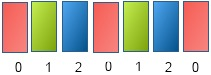
\includegraphics{rand7mod3}
  \caption{Low number bias of a random number generator taken module.}
  \label{fig:rand7mod3}
\end{figure}

\index{random numbers!generator!C language|)}

\Level 1 {C++}
\index{random numbers!generator!C++ language|(}
\lstset{language=C++}

The \ac{STL} has a
\indextermbus{random number}{generator}
that is more general and more flexible than the C~version.
\begin{itemize}
\item There are several generators that give uniformly distributed
  numbers;
\item then there are distributions that translate this to non-uniform
  or discrete distributions.
\end{itemize}

First you declare an engine; later this will be transformed into a distribution:
\begin{lstlisting}
std::default_random_engine generator;
\end{lstlisting}

This generator will start at the same value every time.
You can seed it:
\begin{lstlisting}
std::random_device r;
std::default_random_engine generator{ r() };
\end{lstlisting}

Next, you need to declare the distribution.
For instance, a uniform distribution between given bounds:
\begin{lstlisting}
std::uniform_real_distribution<float> distribution(0.,1.);
\end{lstlisting}
A roll of the dice would result from:
\begin{lstlisting}
std::uniform_int_distribution<int> distribution(1,6);
\end{lstlisting}

\Level 2 {Random floats}

\begin{lstlisting}
// seed the generator
std::random_device r;
// std::seed_seq ssq{r()};
// and then passing it to the engine does the same

// set the default random number generator
std::default_random_engine generator{r()};

// distribution: real between 0 and 1
std::uniform_real_distribution<float> distribution(0.,1.);

cout << "first rand: " << distribution(generator) << endl;
\end{lstlisting}

\Level 2 {Dice throw}

\begin{lstlisting}
// set the default generator
std::default_random_engine generator;

// distribution: ints 1..6
std::uniform_int_distribution<int> distribution(1,6);

// apply distribution to generator:
int dice_roll = distribution(generator);
  // generates number in the range 1..6 
\end{lstlisting}

\Level 2 {Poisson distribution}

  Another distribution is the \indextermbus{Poisson}{distribution}:
\begin{lstlisting}
std::default_random_engine generator;
float mean = 3.5;
std::poisson_distribution<int> distribution(mean);
int number = distribution(generator);
\end{lstlisting}

\index{random numbers!generator!C++ language|)}

\Level 1 {Fortran}
\index{random numbers!generator!Fortran language|(}
\lstset{language=Fortran}

In this section we briefly discuss the Fortran \emph{random number generator}.
The basic mechanism is through the library subroutine
\indextermtt{random_number}, which has a single argument of type
\lstinline{REAL} with \lstinline{INTENT(OUT)}:
\begin{lstlisting}
real(4) :: randomfraction
call random_number(randomfraction)
\end{lstlisting}
The result is a random number from the uniform distribution
on~$\left[0,1\right)$.
  
Setting the \indextermbus{random}{seed} is slightly convoluted. The
amount of storage needed to store the seed can be processor and
implementation-dependent, so the routine \indextermtt{random_seed}
can have three types of named argument, exactly one of which can be
specified at any one time. The keyword can be:
\begin{itemize}
\item \lstinline{SIZE} for querying the size of the seed;
\item \lstinline{PUT} for setting the seed; and
\item \lstinline{GET} for querying the seed.
\end{itemize}
A typical fragment for setting the seed would be:
\begin{lstlisting}
integer :: seedsize
integer,dimension(:),allocatable :: seed

call random_seed(size=seedsize)
allocate(seed(seedsize))
seed(:) = ! your integer seed here
call random_seed(put=seed)
\end{lstlisting}

\index{random numbers!generator!Fortran language|)}

\Level 1 {Python}
\index{random numbers!generator!Python language|(}
\lstset{language=Python}
\index{random numbers!generator!Python language|)}

Python has a random module:
\lstset{language=Python}
\begin{lstlisting}
import random
x = random.random()
i = random.randint(lo,hi)
\end{lstlisting}
\lstset{language=C}

\Level 0 {Parallel random number generation}
\label{sec:parallel-random}
\index{random numbers!generator!parallel|(}

Random number generation is problematic in parallel. To see this,
consider a parallel process that uses a random number generator on
each subprocess, and
consider a single processor emulating the parallel process. Now this
single process in effect has a random number generator that consists
of interleaving the parallel generator results. This means that, if we
use the same generator in all parallel processes, the effective
generator over the whole process will produce stretches of identical
values.

There are various ways out.

\Level 1 {Manager-worker generator}

We can generate the random numbers centrally. In shared memory that could mean
making its operation atomic. This may introduce a serious bottleneck.
\begin{exercise}
  Critical sections are usually justified if the work spent there is of lower order
  than the parallel work. Why does that argument not apply here.
\end{exercise}

Another solution would be to have one thread or process that generates
the random numbers and distributes them to the other processes.
Doing this on a number-by-number basis causes considerable overhead.
Instead, it would be possible for the generator process to distribute
blocks of numbers. However, the manner in which this is done may again
cause correlation between processes.

\Level 1 {Sequence splitting solutions}

A~better solution is to set up independent generators with
parameter choices that guarantee statistical randomness. This is not
simple. For instance, if two sequences $x^{(1)}_i,x^{(2)}_i$ have the
same values of $a,b,m$, and their starting points are close together,
the sequences will be strongly correlated. Less trivial examples of
correlation exist.

Various techniques for random number generation exist, such as using
two sequences, where one generates the starting points for the other
sequence, which is the one actually used in the simulation. Software
for parallel random number generator can be found at
\url{http://sprng.cs.fsu.edu/}~\cite{Mascagni:SPRNG}.

If it is possible given $x_i$ to compute $x_{i+k}$ cheaply, one use a
leapfrogging technique, where $k$ processes have disjoint series
$i\mapsto x_{s_k+ik}$ where $x_{s_k}$ is the starting point for the
$k$-th series.

\Level 1 {Blocked random number generators}

Some random number generators (see~\cite{LEcuyer:multiple-random})
allow you to calculate a value that is many iteration away from the seed.
You could then take the block of values from the seed to that iteration
and give it to one processor. Similarly, each processor would get a contiguous
block of iterations of the generator.

\Level 1 {Keyed random number generators}

Some random number generators are not recursive, but allow
an explicit formulation \[ x_n = f(n), \]
that is, the $n$-th number is a function of its `key',~$n$.
Adding a block key into the equation
\[ x_n^{(k)} = f_k(n) \]
allows for parallelism over processes indexed by~$k$.
See~\cite{Salmon:prng123}.

\Level 1 {Mersenne twister}

The \indexterm{Mersenne twister} random number generator has been
adapted to allow for parallel streams of uncorrelated
numbers~\cite{Matsumoto:DynamicMersenne}. Here the process ID is
encoded into the generator.

\index{random numbers|)}
\index{random numbers!generator!parallel|)}


% LocalWords:  Eijkhout Monte Carlo rand int srand ssq cout endl ints
% LocalWords:  randomfraction seedsize allocatable leapfrogging
% LocalWords:  Mersenne
